\documentclass[english,course]{lecture}

\usepackage{minted}
\usepackage{hyperref}
\usepackage{caption}
\usepackage{graphicx}
\graphicspath{ {./images/} }

\title{MongoDB intro}
\attn{I kan finde kildekoden (skrevet i \LaTeX) til disse lecture notes på github - I er velkomne til at kommentere der hvis i finder fejl eller noget der kunne forklares bedre \url{https://github.com/janmeier/cbs-lecture-notes}}
\author{Jan Aagaard Meier}
\email{jam.digi@cbs.dk}

\newminted{bash}{}
\newminted{js}{linenos,tabsize=2,breaklines}
\newmintinline{js}{}
\newmintinline{sql}{}
\renewcommand{\listingscaption}{Eksempel}
\usepackage[figurename=Figur]{caption}

\RequirePackage{accsupp}
\renewcommand\theFancyVerbLine{
    \BeginAccSupp{method=escape,ActualText={}}
    {\rmfamily\tiny\arabic{FancyVerbLine}}
    \EndAccSupp{}

}

\begin{document}

\section{Installation}
Start med at installere mongo serveren fra \url{https://docs.mongodb.com/manual/administration/install-community/}. 

Derefter skal du installere mongodb, som er det node.js bibliotek vi bruger til at snakke med mongo. Det skal installeres i den mappe hvor resten af jeres kode ligger (for at holde tingene adskilt kan i eventuelt oprette en server mappe til database og server koden i jeres projektmappe). I terminalen (terminal på linux / OSX, Git bash på Windows) skriver i følgende:

\begin{minted}{bash}
npm install mongodb
\end{minted}

Derefter er det tid til at test at der er hul igennem til databasen - Det gør i med et kort stykke kode: 

\begin{listing}[H]
\caption{Test af forbindelsen til databasen}
\label{lst:testconnection}
\begin{jscode}
const MongoClient = require('mongodb').MongoClient;

// Connection URL
const url = 'mongodb://localhost:27017';
const dbName = 'myproject';

const client = new MongoClient(url);

client.connect().then(() => {
  console.log("Connected successfully to server");

  const db = client.db(dbName);

  client.close();
});
\end{jscode}
\end{listing}

I kan fx gemme det i en fil ved navn \mintinline{bash}{test.js} og køre \mintinline{bash}{node test.js} i terminalen.

På linje 5-6 fortæller vi hvordan der skal forbindes til vores mongo server. \jsinline/mongodb:/// er protokollen vi bruger til at kommunikere med mongo serveren, på samme måde som http(s) er den protokol vi bruger til at snakke med en webserver.
 \ jsinline/localhost/ fortæller at mongo kører på samme computer som vores node script, mens \jsinline/:27017/ fortæller hvilken port vi skal forbinde til.

Hvis I har gjort alt rigtig bør i se noget i stil med dette i terminalen:

\begin{bashcode}
Connected successfully to server
\end{bashcode}

\section{Database setup}
\subsection{Intro}

I mongodb biblioteket er connection pooling indbygget - Vi behøver altså ikke eksplicit at importere eller instantiere en pool. Ligesom med postgres er det vigtigt at i \textit{ikke} kalder \jsinline/client.end()/ efter hver query som i eksempel \ref{lst:testconnection}.

I de følgende eksempler antages det er \jsinline/db/ variablen er tilgængelig, så vi definerer den ikke hver gang. I jeres eget projekt giver det heller ikke mening at lave en ny client eller db instans i hver fil hvor i skal bruge den. I stedet kan i definere den i een fil, eksportere den og så \jsinline/require/ den de steder den skal bruges:

\begin{listing}[H]
\caption{db.js}
\begin{jscode}
const MongoClient = require('mongodb').MongoClient;
const url = 'mongodb://localhost:27017';
const dbName = 'myproject';
const client = new MongoClient(url);

function getDb() {
	return client.connect().then(() => {
		return client.db(dbName);
	});	
}

module.exports = getDb;
\end{jscode}
\end{listing}

Til forskel fra postgres er vi med mongodb nødt til at kalde \jsinline/connect()/ før vi kan få en instans af db klassen, som er den vi bruger til at arbejde med databasen. \jsinline/connect()/ er et asynkront kald, fordi vi skal en tur over netværket (selvom jeres mongodb server er på samme computer) for at hente data. Hver gang i har brug for en db instans er i derfor nødt til at kalde funktionen \jsinline/getDb/. I alle følgende eksempler, antages det at \jsinline/getDb/ allerede er kaldt, og at \jsinline/db/ variablen er tilgængelig.

\begin{listing}[H]
\caption{user.js}
\begin{jscode}
const getDb = require('./db');

getDb().then(db => {
	// do something with db here
})
\end{jscode}
\end{listing}


\subsection{Tabeller}
I postgres snakker vi om rækker af data, og disse rækker er samlet i en tabel. Da mongo er en dokumentdatabase er hvert stykke data et dokument, og disse dokumenter er samlet i en collection. I praksis er både rækker og dokumenter repræsenteret som et JSON objekt i javascript.


\subsubsection{Skemaer og datamodellering}
Den store forskel på dokumentdatabaser og relationelle databaser er hvor strikse de er omkring at det data der indsættes skal overholde det skema der er defineret. I en relationel database \textit{skal} vi definere skemaet før vi overhovedet får lov at indsætte data. Dette gøres med \sqlinline/CREATE TABLE/ statements, som præcist beskriver hvilke attributter dataen har, og hvilke datatyper de har. 
I mongodb er det muligt, men ikke påkrævet at definere et skema. Skemaet kan også tilføjes efter at der allerede er tilføjet data til en collection. Endelig er der i mongodb mulighed for at aktivt at vælge at ignorere skemaet efter at det defineret, hvilket ikke er muligt i postgres.\margintext{For mere om skema validering i mongo, se \url{https://docs.mongodb.com/manual/core/schema-validation/}}

Da postgres er en relationel database, har man mulighed for at definere relationer som en del af sit skema. Hvis man fx har to tabeller, customer og order, og order indeholder customer\_id, kan vi definere i skemaet for order, at customer\_id refererer til en række i customer tabellen, således at der ikke kan oprettes en ordre for en kunde som ikke findes. Vi kan godt modellere det samme skema i mongodb med en customer og en order collection, men det er ikke muligt at få mongo til at validere at alle ordrer tilhører en kunde. 

Generelt snakker vi om to måder at bygge datamodeller på, de kan være enten \textbf{normaliserede} (eksempel \ref{lst:normalized}), eller \textbf{indlejrede} (embedded, eksempel \ref{lst:embedded}). De to følgende eksempler viser hvordan datamodellen i figur \ref{fig:er} kan modelleres som henholdsvis normaliseret og indlejret.

\begin{figure}[H]
\caption{Én kunde har mange ordrer}
\label{fig:er}
\centering
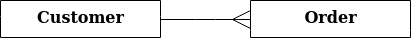
\includegraphics[width=0.5\textwidth]{er}
\end{figure}

\begin{listing}[H]
\caption{Normaliseret kunde-ordre relation. Læg mærke til at hver }
\label{lst:normalized}
\begin{jscode}
const customers = [{
	id: 42,
	name: "Foo"
}];

const orders = [{
	user_id: 42,
	total_amount: 53.4
}]
\end{jscode}
\end{listing}

\begin{listing}[H]
\caption{Indlejret kunde-ordre relation}
\label{lst:embedded}
\begin{jscode}
const customers = [{
	id: 42,
	name: "Foo",
	orders: [{
		total_amount: 53.4
	}]
}];
\end{jscode}
\end{listing}

Nogle relationelle databaser har mulighed for at definere en kolonne af typen \sqlinline/JSON/, således at man kan indlejre data i sine tabeller, men i min erfaring fra mit professionelle arbejde benytter mindst 90\% af alle relationelle databaseskemaer sig af et normaliseret design. Dokumentdatabaser associeres oftest med et indlejret skemadesign, men har altså mulighed for begge dele.

Der er ikke nogle håndfaste regler for hvornår det giver mening at benytte det ene eller det andet, men der er dog nogle overordnede guidelines. Se linket i margenen for flere detaljer. Hvis i vælger mongodb gør i altså en bevidst valg om hvorvidt i laver jeres datamodel normaliseret eller indlejret (eller en kombination). Husk at argumentere for dette valg i jeres rapport. \margintext{For mere om datamodellering i mongo, se \url{https://docs.mongodb.com/manual/core/data-model-design/}}

\\\textbf{Grunde til at vælge indlejret}

\begin{itemize}
	\item Når der er en klar 1:1 relation mellem dataen, og parent-dokumentet "ejer" child-dokumentet. Det kunne fx være user og address - Brugeren ejer adressen (selvfølgelig kan flere brugere have samme addresse, men det vil ske meget sjældent)
	\item Ved 1:mange relationer hvor child-dokumentet altid vises eller bruges i kontekst af dets parent. Det kunne fx være et brugersystem, hvor hver bruger kan tildeles mange roller. Her har vi næsten altid brug for at indlæse brugerens roller, for at kunne se hvad han har adgang til i systemet
	\item Generelt giver indlejret bedre performance ved læsninger, da man kan hente alt det data man skal bruge i een operation, i stedet for at skulle kigge i flere collections. Dette gør sig selvfølgelig kun gældende, hvis man faktisk skal bruge den data man henter. Hvis man henter et langt array af child-dokumenter for et parent-dokument, men kun bruger dem hver 10. gang er der ikke nogen besparelse ved at indlejre dataen.
\end{itemize}

\\\textbf{Grunde til at vælge normaliseret}

\begin{itemize}
	\item Ved 1:mange relationer hvor parent-dokumentet har mange child-dokumenter (som regel flere hundrede). Mongodb har en grænse for hvor stort et enkelt dokument kan være, og hvis vi gemmer mange hundrede child-dokumenter på et parent-dokument rammer vi hurtigt den grænse. Ydermere vil det være tungt at skulle hente flere hundrede child-dokumenter hver gang vi skal hente en parent
	\item Ved 1:mange relationer hvor vi ønsker at kunne vise (og måske opdatere) child-dokumenter uafhængigt af deres parent. Det kan fx være at man i kunde / ordre relationen fra figur \ref{fig:er} ønsker at vise en liste af alle ordrer. Her giver det mening af kunne kigge direkte ned i en order collection, i stedet for at skulle løbe alle kunder igennem for at finde deres ordrer
	\item Ved mange:mange relationer, for at undgå duplikering af data. Forestil dig relationen mellem bruger og event - mange brugere kan være tilmeldt det samme event, og en bruger kan tilmelde sig mange events. I dette tilfælde giver det ikke mening at gemme events på hver bruger, da vi så vil opbevare det samme data (sted, tidspunkt osv.) mange gange, hvilket også vil gøre det svært at opdatere et event, fordi man så skulle opdatere for hver bruger der er tilmeldt
\end{itemize}

Så længe i argumenterer godt for jeres design kan i i langt de fleste tilfælde slippe afsted med begge valg.

\section{Queries}

\subsection{Read}
Hvor man i SQL skriver sine queries som tekst, beskrives queries i mongodb som javacript objekter. I den simpleste form bruger et objekt til at beskrive præcis hvilken værdi man vil have.

\begin{listing}[H]
\caption{I en normaliseret databasemodel, find brugeren med email jam.digi@cbs.dk, og find alle hans ordrer. Læg mærke til at id er prefixet med underscore}
\begin{jscode}
db.collection('users').findOne({
	email: 'jam.digi@cbs.dk'
}).then(user => {
	db.collection('orders').find({
		user_id: user._id
	}).toArray().then(orders => {
		// Do something with the orders
	});
});
\end{jscode}
\end{listing}

For mere avancerede queries bruger vi \textit{operatorer} (kan fx være 'større end', 'eller' osv.), som prefixes med et dollartegn. For at finde alle brugere som har emailen jam.digi@cbs.dk, eller har en mail som slutter på gmail.com kan vi bruger \jsinline/$or/ operatoren. \margintext{Se \url{https://docs.mongodb.com/manual/tutorial/query-documents/} og \url{https://docs.mongodb.com/manual/reference/operator/query/\#query-selectors} for flere eksempler}

\begin{listing}[H]
\caption{Find alle brugere med som har emailen jam.digi@cbs.dk, eller en email som slutter på gmail.com}
\begin{jscode}
db.collection('users').find({
	$or: [{ email: 'jam.digi@cbs.dk'}, { email: { $regex: /gmail.com$/ }}]
}).toArray().then(users => {
	// Do something with the users
});
\end{jscode}
\end{listing}

\subsection{Insert}

For at indsætte et dokument i en collection kalder du \jsinline/insertOne/ funktionen med et objekt. Result-objektet indeholder \jsinline/ops/, som er et array af de dokumenter der er blevet indsat, mens \jsinline/insertedIds/ indeholder id for dokumenterne.

\begin{listing}[H]
\begin{jscode}
db.collection('users').insertOne({
	email: 'jam.digi@cbs.dk'
}).then(result => {
	console.log(result)
	/*
		{
		  result: { ok: 1, n: 1 },
		  ops: [ { email: 'jam.digi@cbs.dk', _id: 5e70cba3aaa9734ff4e5d83b } ],
		  insertedCount: 1,
		  insertedIds: { '0': 5e70cba3aaa9734ff4e5d83b }
		}
	*/
})
\end{jscode}
\end{listing}

For at indsætte flere dokumenter samtidig kan du bruge \jsinline/insertMany/, og kalde funktionen med et array af objekter. Outputformatet er det samme som for \jsinline/insertOne/.

\subsection{Update}

For at opdatere et eller flere dokumenter kaldes funktionerne \jsinline/updateOne/ eller \jsinline/updateMany/ med to objekter. Det første fortæller \textit{hvilke} dokumenter der skal opdateres, og har samme format som det der bruges til find. Det andet objekt fortæller \textit{hvordan} dokumenterne skal opdateres.

\begin{listing}[H]
\caption{Opdater brugeren med email jam.digi@cbs.dk password til qwerty123}
\begin{jscode}
db.collection('users').updateOne({
	email: 'jam.digi@cbs.dk'
}, {
	password: 'qwerty123'
}).
\end{jscode}
\end{listing}

\begin{listing}[H]
\caption{Opdater alle ordrer hvor user\_id er 42 eller 43 til shipped}
\begin{jscode}
db.collection('orders').updateMany({
	user_id: { $in: [42, 43] }
}, {
	shipped: true
}).
\end{jscode}
\end{listing}

\end{document}